\epigraph{To doubt everything or to believe everything are two equally convenient solutions; both dispense with the necessity of reflection.}
{\textit{Henri Poincaré}}

\section{First Year Mathematics Workshops}

\subsection{Introduction to Workshops}

Maths Workshops are interactive and supportive sessions that are designed to help students mainly with coursework and classes, but  welcome students to come and ask questions about any aspect of the maths. These are held daily in the \textbf{\href{https://www.southampton.ac.uk/study/facilities/maths-study-social-spaces}{Maths Student Centre}} and the timetable for them is published on Blackboard once the semester starts. First year students can get help from the member of staff present there or any of the designated `workshop helpers', who are usually third-year or postgraduate students. 

\subsection{More Than Just Coursework Help}

When I first started, I thought the first year workshops were basically just getting help for your coursework and nothing else. But the biggest difference I noticed was that when I genuinely struggled with a problem, even if I got nowhere, the workshop became the most valuable resource. 

If you go hoping someone will just show you the solution from scratch, you leave having learned much less than you could have. Even 15 minutes of serious attempt make major impact as it makes you aware of where you're stuck, and gives you something specific to ask about. 

% talk about how I got to know older students via workshops, and how useful it is to just go there and chat to staff and older studnets too. I think we're really lucky as a dept. to have this cuz some unis' don't give a fuck about thier students. 

\section{AI and Outsourcing Thinking}

It would be highly ignorant and unrealistic of me to not talk about Generative AI. We all know it exists and it can generate solutions instantly. And sometimes, it is useful, it can clarify notation or rephrase definitions and help fill in some gaps in reasoning.

However, the biggest drawback of AI is that it removes the part of the process that actually builds the understanding. If you ask AI to generate a full solution to a problem you haven't seriously attempted, you might feel productive, even pleased looking at the solution, but you've just skipped the uncomfortable but crucial bit where your brain learns by trying, failing, and reattempting ideas. And that's the uncomfortable bit where understanding takes place. 

GenAI is very good at doing things, so it’s tempting to just ask it for answers. But imagine training for a marathon with a personal trainer. You wouldn’t expect your trainer to do all the running and training for you and then expect yourself to perform well on race day. Their role is to challenge you, guide you, and help you get stronger.

Generative AI should be used in the same way. There is a difference between using AI to complement your learning, and using it to replace your work and your thinking entirely, and it is important that you be honest with yourself about which one you're doing. At the end of the day, you are the one being impacted by your use/misuse of AI, so take accountability. 

The department and the university has its own policy on AI, so I urge you to read it because it matters not only due to academic integrity, but because this degree is about learning to think independently. 
% There are univeristy and department policies on AI, add links to them so that I don't end up saying something that will be hugley incorrect? 

\section{Other Resources}

Alongside lectures and problem sheets, there are a number of external resources that can help clarify ideas or offer a different perspective. This is not an exhaustive list, just a few that I’ve found useful.

\subsection{YouTube Channels}

% lots of good youtube channels for maths + developing general interest 
% youtube videos, suggested links? some that helped me... compile a list 

% Michael Penn, Trefor Bazett, 3b1b, Numberphile 

% WHAT ARE TEXTBOOKS/IS THERE A MODULE READING LIST? - add link to that 


\begin{figure}[H]
    \centering
    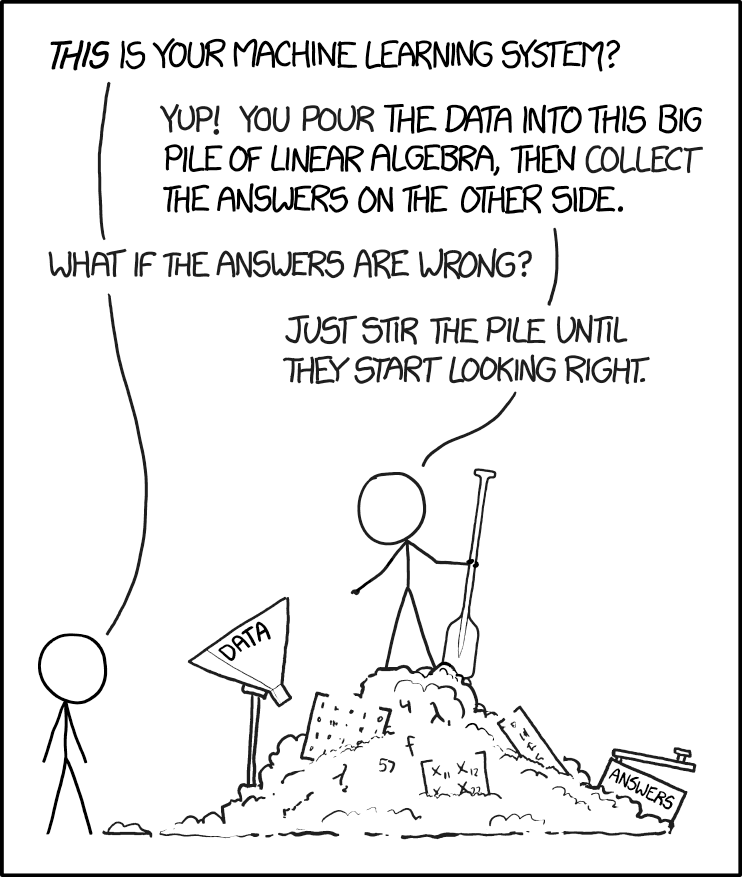
\includegraphics[width=0.5\linewidth]{xkcd/MachineLearning.png}
    \caption{\textbf{\href{https://xkcd.com/1838/}{Machine Learning}}}
\end{figure}